\documentclass[12pt]{article}
\usepackage[utf8]{inputenc}
\usepackage[usenames]{color}
\usepackage[margin=1in]{geometry} 
\usepackage{amsmath,amsthm,amssymb,graphicx,mathtools,tikz,hyperref, pgfplots, listings, pdfpages}
\usetikzlibrary{positioning}
\newcommand{\n}{\mathbb{N}}
\newcommand{\z}{\mathbb{Z}}
\newcommand{\q}{\mathbb{Q}}
\newcommand{\cx}{\mathbb{C}}
\newcommand{\real}{\mathbb{R}}
\newcommand{\field}{\mathbb{F}}
\newcommand{\ita}[1]{\textit{#1}}
\newcommand{\com}[2]{#1\backslash#2}
\newcommand{\oneton}{\{1,2,3,...,n\}}
\newcommand\idea[1]{\begin{gather*}#1\end{gather*}}
\newcommand\ef{\ita{f} }
\newcommand\eff{\ita{f}}
\newcommand\proofs[1]{\begin{proof}#1\end{proof}}
\newcommand\inv[1]{#1^{-1}}
\newcommand\setb[1]{\{#1\}}
\newcommand\en{\ita{n }}
\newcommand{\vbrack}[1]{\langle #1\rangle}


\newenvironment{theorem}[2][Teorema]{\begin{trivlist}
\item[\hskip \labelsep {\bfseries #1}\hskip \labelsep {\bfseries #2.}]}{\end{trivlist}}
\newenvironment{lemma}[2][Lema]{\begin{trivlist}
\item[\hskip \labelsep {\bfseries #1}\hskip \labelsep {\bfseries #2.}]}{\end{trivlist}}
\newenvironment{exercise}[2][Ejercicio]{\begin{trivlist}
\item[\hskip \labelsep {\bfseries #1}\hskip \labelsep {\bfseries #2.}]}{\end{trivlist}}
\newenvironment{reflection}[2][Reflexión]{\begin{trivlist}
\item[\hskip \labelsep {\bfseries #1}\hskip \labelsep {\bfseries #2.}]}{\end{trivlist}}
\newenvironment{proposition}[2][Proposición]{\begin{trivlist}
\item[\hskip \labelsep {\bfseries #1}\hskip \labelsep {\bfseries #2.}]}{\end{trivlist}}
\newenvironment{corollary}[2][Corolario]{\begin{trivlist}
\item[\hskip \labelsep {\bfseries #1}\hskip \labelsep {\bfseries #2.}]}{\end{trivlist}}
 \hypersetup{
 colorlinks,
 linkcolor=blue
 }

\renewcommand{\ttdefault}{pcr}
\lstdefinestyle{C}{language=C,
    basicstyle=\ttfamily,
    keywordstyle=\bfseries,
    showstringspaces=false,
    morekeywords={include, printf},
	keepspaces=true,numbers=left,xleftmargin=2em,frame=shadowbox,framexleftmargin=0 em, rulesepcolor = \color{black}
}
\lstdefinestyle{linuxterminal}{language=bash,
    basicstyle=\ttfamily,
    keywordstyle=\bfseries,
    showstringspaces=false,
    morekeywords={include, printf},
	keepspaces=true,
	frame=TLRB
}


\begin{document}
	\date{05-04-2018}
	
	
	\title{\textbf{\textcolor{red}{CODING AND TESTING REPORT}}}
	\author{Alejandro Santorum Varela - alejandro.santorum@estudiante.uam.es\\David Cabornero Pascual - david.cabornero@estudiante.uam.es\\Universidad Autónoma de Madrid}
	\maketitle
	
	\tableofcontents
	
	\newpage

\section{Introduction}
We are right now in the first coding phase of the project. This little small report tries to give a brief of the principal decisions and guide the reader through the practice material.\\

\section{Source Code and Javadoc}
In the folder of the assignment we have placed a sub-folder called \textbf{project} which contains all the programmed packages: Exceptions, Filters, Testers and padsof(where the main source code of the app is placed).\\\\
In the first package we include all the programmed exceptions, created in order to simplify the error control and manage the different incorrect data stream.\\\\
The Filters package contains the interface \emph{Filter} and the different filters that implements it, one per different search that our application is capable of perfoming.\\\\
Testers package is where all the testing code of the application is saved. All of them but two are JUnit tests, one per class.\\ The unity test of classes checks every functionality of the class, \textbf{testing all the methods and possible mistakes}. Comment that the unity test of the  \emph{Application class} can be considered as a integration test. However, we have programmed another two testings: one is the considered "InitialTester" that checks rapidly the main functionality of the application methods, and the last one, that is the "IntegrationFinalTest", that is a demo of every action that the application can develop. It's important to remember that small actions (like blocking an user using setBlocked() method of RegisteredUser class) are mainly shown in the unity tests using JUnit.\\\\
Finally, the padsof package is where all the classes that model the application are placed.\\\\
Moreover, in this same folder we include the \texttt{Javadoc documentation}, you can check it if something about the design is not clear\\.
	
\section{Class Diagram}
Here we show the new class diagram after some changes during the coding phase. Due to the fact is difficult to see every word in this class diagram, we have provided it in the assignment folder as well:
\begin{center}
	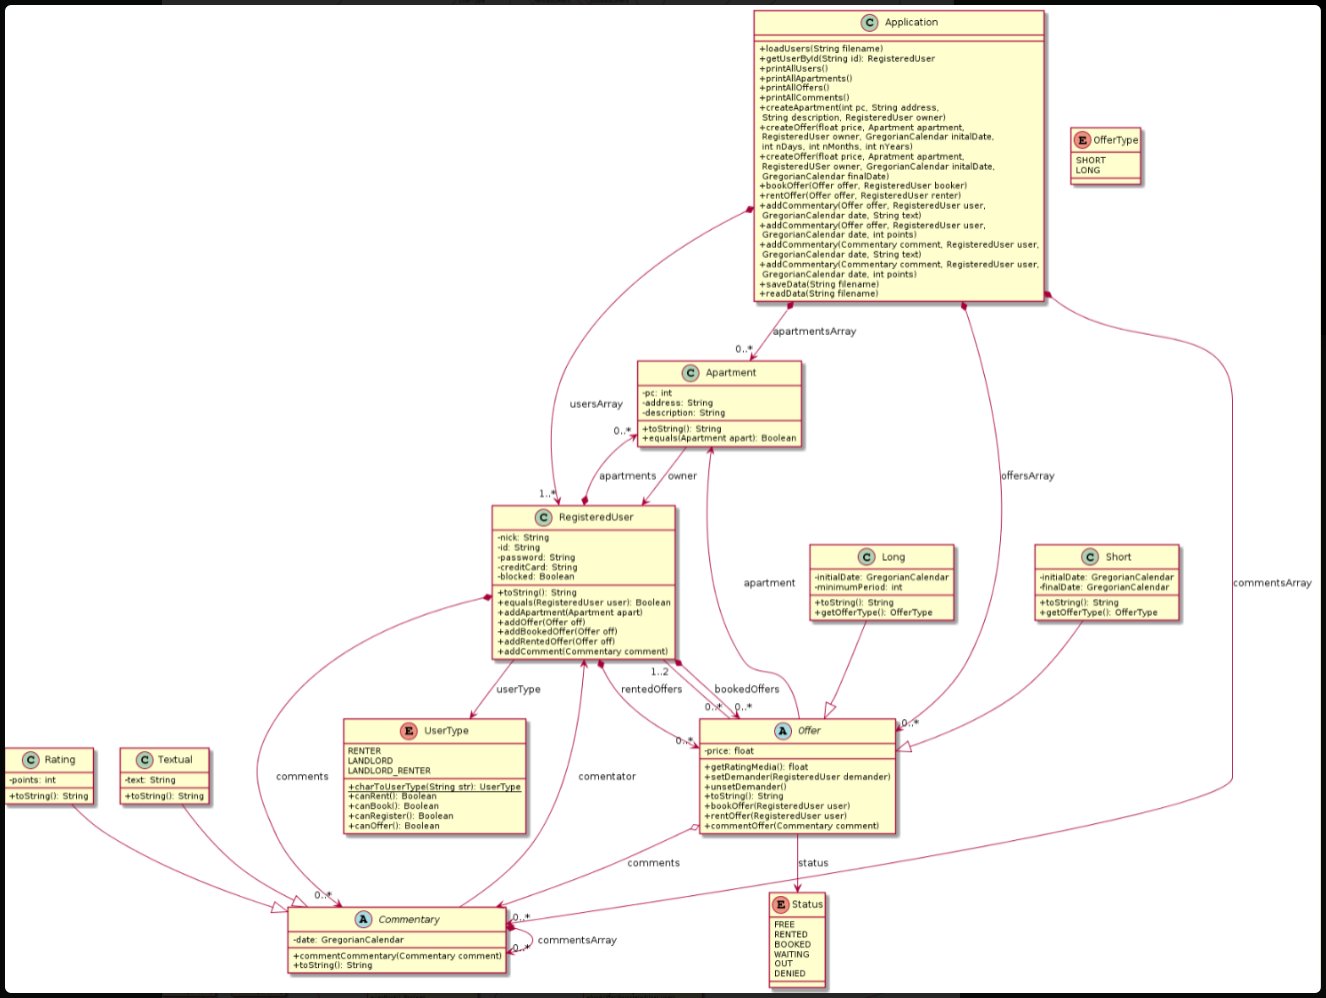
\includegraphics[scale=1]{ClassDiagram.PNG}
\end{center}
The first thing we have to keep in mind is that exceptions and filters are not shown here becuase they are not related directly. Just below we attach some graphics to indicate the relationship between the different exceptions and the filters.
\begin{center}
	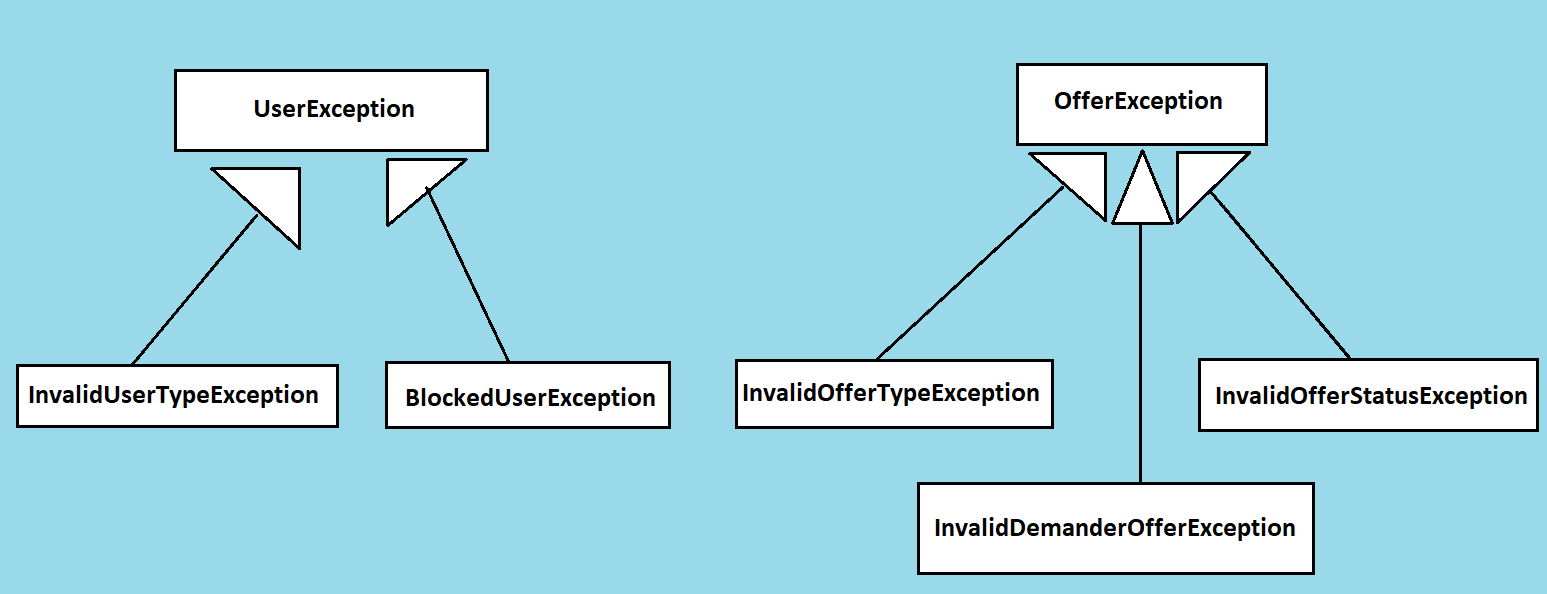
\includegraphics[scale=0.8]{ExceptionsGraphic.PNG}
\end{center}
\begin{center}
	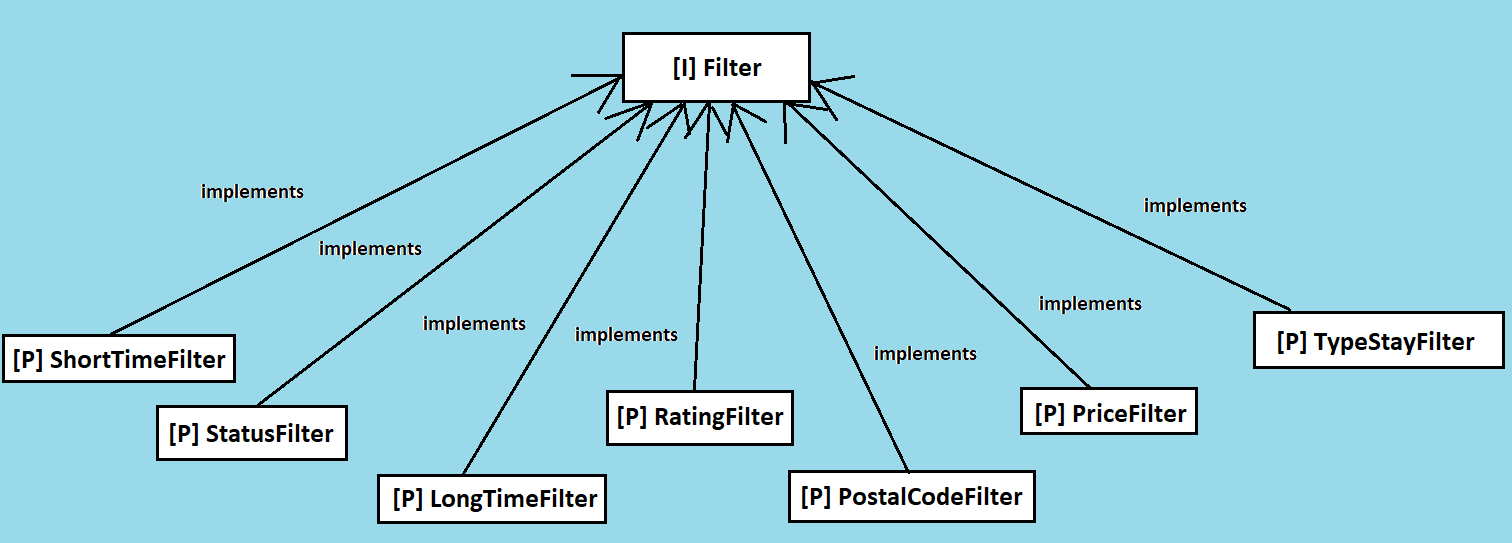
\includegraphics[scale=0.8]{FiltersGraphic.PNG}
\end{center}
In the FIlters graphic [P] means public class and [I] means interface. So every filter class implements the filter interface.\\


\section{Traceability Matrix}
The traceability matrix are divided in four different files because of its huge size. All of this files are included in the assignment folder, in one folder called "Traceability matrix".\\\\
There is nothing to comment about that. Just say the difference between this matrix and the previous one, is quite meaningful, the improvement is visible.\\

\section{Conclusion}
This is one of the most difficult practices and thats why it is the most valuable one. However, we think we have done a good job developing and implementing every requested functionality.\\\\
If there is any doubt just email us.
	
	
\end{document}